% !TeX root = ../../../../thesis.tex

\subsection{DC}
\label{subsec:dc-testbed-eval}

The DC testbed has six LEDs, as explained in \autoref{subsec:dc-testbed}.
Therefor six IDs will be used for the LEDs with a seventh code used to represent an LED in an off state.
From \autoref{tbl:correlation-gold-families}, we can see that for $m = 6$, where $m$ is the number of simultaneous transmitters such that no destructive interference takes place, requires a code length of 511 or higher.
With the DC testbed the experiments have been performed with a constant modulation frequency of 1 kHz.
Every two successive samples are $\frac{1}{1000} = 1$ ms apart.

In \autoref{fig:raw-dc-testbed-adc-data-n=9} the raw ADC data from the DC testbed can be seen.
The left y-axis represents the raw ADC data and the right y-axis is converted to current.
Six LEDs are continuously and simultaneously modulating with different starting times.
From the figure, seven horizontal lines can be seen.
Each line represents how many LEDs are on: When all LEDs are encoding a `0', the current will also be zero, when only one of the six LEDs is encoding a `1' the current is roughly 50 mA, when exactly two LEDs are encoding a `1', the current is roughly 100 mA, and so on.
In contrast to the AC case which will be explained in the next section, in the DC case there is only positive current and no trigger signals to consider, so this raw data is already in a form for which we can start calculating the correlation for the ID of an LED.

\begin{figure}[t]
  \centering
  \begin{minipage}[b]{0.49\textwidth}
    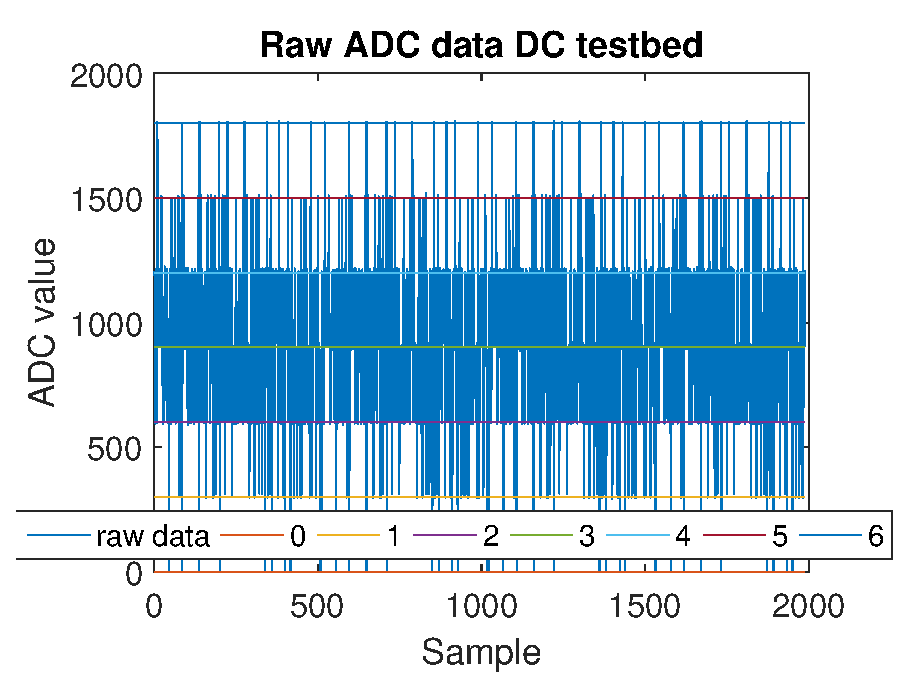
\includegraphics[width=\textwidth]{chapters/evaluation-chapters/hardware/dc/raw-dc-testbed-adc-data-n=9.eps}
    \caption{Raw ADC data from the DC testbed. With seven distinguishable entries, following the on-state of the combinations of LEDs. With a sequence length of 511.}
    \label{fig:raw-dc-testbed-adc-data-n=9}
  \end{minipage}
  \hfill
  \begin{minipage}[b]{0.49\textwidth}
    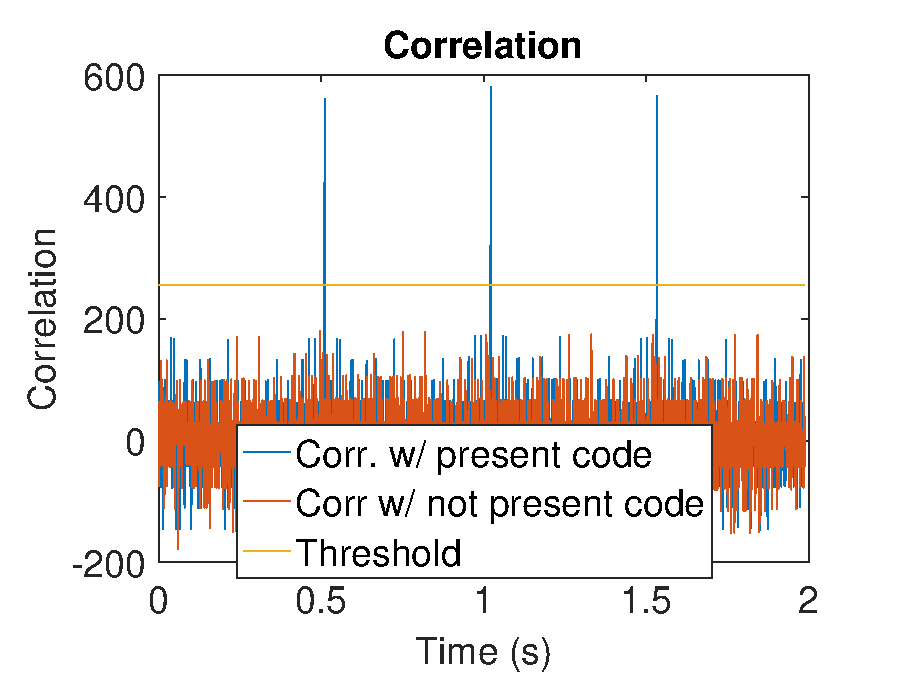
\includegraphics[width=\textwidth]{chapters/evaluation-chapters/hardware/dc/correlation-dc-testbed-n=9.eps}
    \caption{Correlations results from the IDs to identify which LEDs are on and off, with the decision threshold. With a sequence length of 511.}
    \label{fig:correlation-dc-testbed-n=9}
  \end{minipage}
\end{figure}


In \autoref{fig:correlation-dc-testbed-n=9}, three graphs are drawn.
The straight line represents the threshold, which is based on the length of the codes used, see \autoref{sec:interference-solution}.
The other two graphs represent the outcome of the correlation with the ID of two LEDs.
One of those IDs is from an LED which is on and the other ID is from the LED which represents an LED in an off state.
The correlation results from the LED which is in an off state, stay below the threshold for all points in time.
This is a good result, since being below the threshold line means that the corresponding LED is off, which in this case is actually true.

The other correlation result shown in \autoref{fig:correlation-dc-testbed-n=9} comes from the ID which corresponds to an LED which is on and modulating.
The results of this correlation show three noticeable peaks which are above the threshold.
These peaks indicate that the ID is present in the sampled current signal by the smart-meter.
There are three peaks, because the LED is continuously transmitting its ID and the length of the ID in combination with the modulation frequency can be transmitted three times in the two second window.
All the peaks mean the same thing: The ID is present in the sampled current signal.
Since this ID represents an LED which is on, these peaks are correct results as they indicate that the LED is indeed on, which is the case.



The evaluation as discussed above for the DC testbed has been run more than ten times.
And for each time the duration of the run was approximately five minutes.
Each run showed the same results as were shown in \autoref{fig:correlation-dc-testbed-n=9}.
As discussed, all correlation results shown in \autoref{fig:correlation-dc-testbed-n=9} are correct.
This means that there are only true-positives and true-negatives.
So the precision, recall and the F-measure are all equal to $1$ according to \autoref{eq:precision}, \autoref{eq:recall} and \autoref{eq:F-measure}, respectively.


\begin{figure}[t]
  \centering
  \begin{minipage}[b]{0.49\textwidth}
    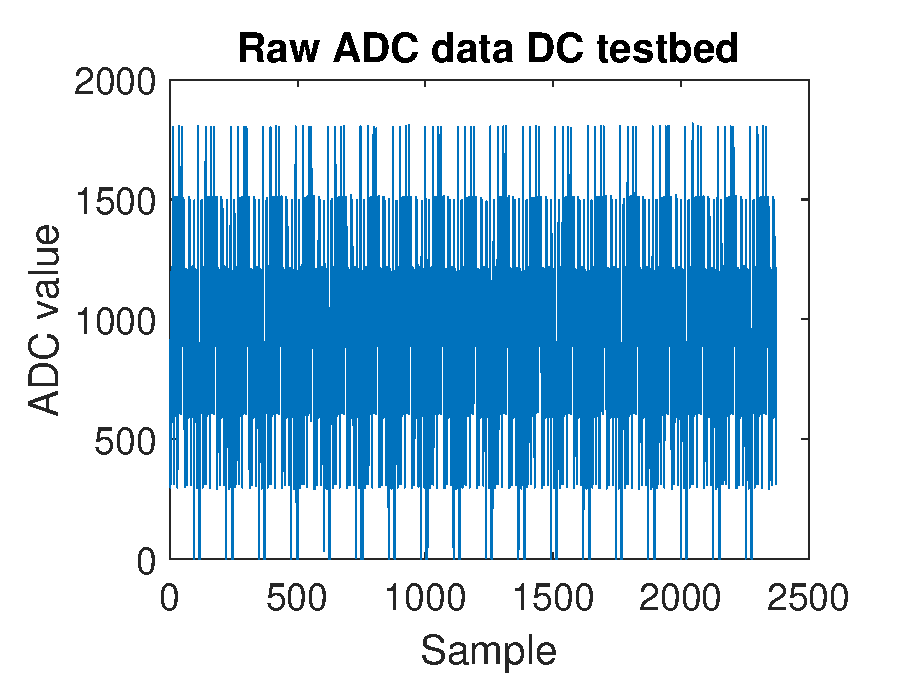
\includegraphics[width=\textwidth]{chapters/evaluation-chapters/hardware/dc/raw-dc-testbed-adc-data-n=7.eps}
    \caption{Raw ADC data from the DC testbed. With seven distinguishable entries, following the on-state of the combinations of LEDs. With a sequence length of 127  on the DC testbed.}
  \label{fig:raw-dc-testbed-adc-data-n=7}
  \end{minipage}
  \hfill
  \begin{minipage}[b]{0.49\textwidth}
    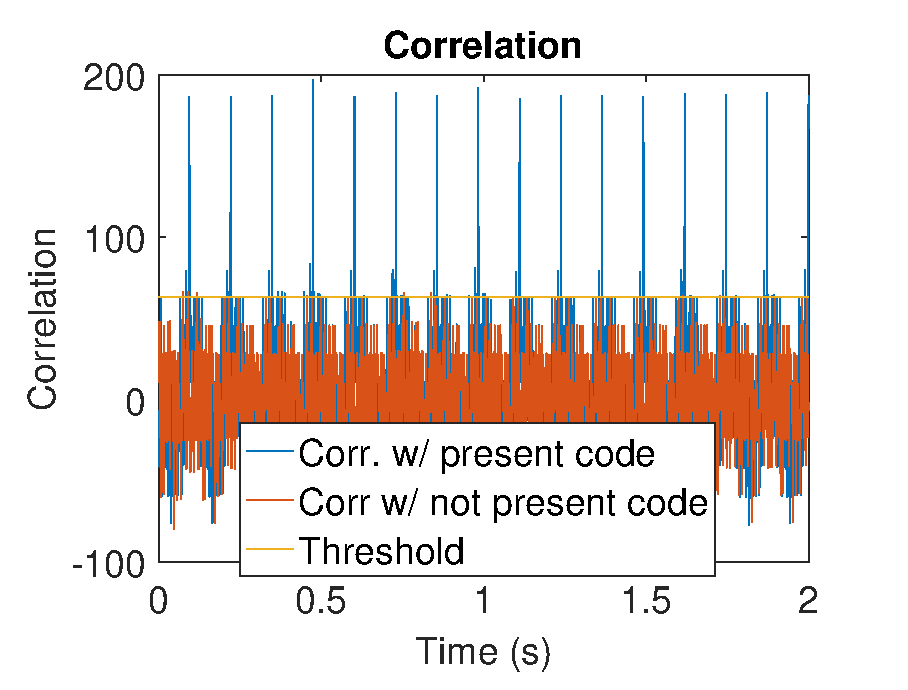
\includegraphics[width=\textwidth]{chapters/evaluation-chapters/hardware/dc/correlation-dc-testbed-n=7.eps}
    \caption{Correlations results from the IDs to identify which LEDs are on and off, with the decision threshold. With a sequence length of 127.}
  \label{fig:correlation-dc-testbed-n=7}
  \end{minipage}
\end{figure}



To show how the accuracy of the system would change when there are false positives and/or false negatives another code length is chosen which does not support six LEDs modulating at the same time.
A length of 127 is chosen, since it may only have three concurrent modulating LEDs (\autoref{tbl:correlation-gold-families}).
Again the six LEDs are continuously and simultaneously modulating with different starting times.
For which the raw ADC data can be seen in \autoref{fig:raw-dc-testbed-adc-data-n=7} on the left y-axis and on the right y-axis the current.
And the correlation results can be found in \autoref{fig:correlation-dc-testbed-n=7}.
In the correlation figure, large peaks can be seen that cross the threshold line, these are the peaks that represent that the ID is present of an LED that is on.
They are supposed to be there, since the LED is actually on.
But also other results can be seen to cross the threshold line.
These are the false-positives, they occur because this code length can not support this many simultaneous LEDs and the interference is too much.
The F-measure in time for these correlation results can be found in \autoref{fig:f-measure-dc-testbed-n=7}.
And the precision, recall and F-measure can be found in \autoref{fig:eval-metrics-dc-testbed-n=7}.





\begin{figure}[ht]
  \centering
  \begin{minipage}[b]{0.49\textwidth}
  	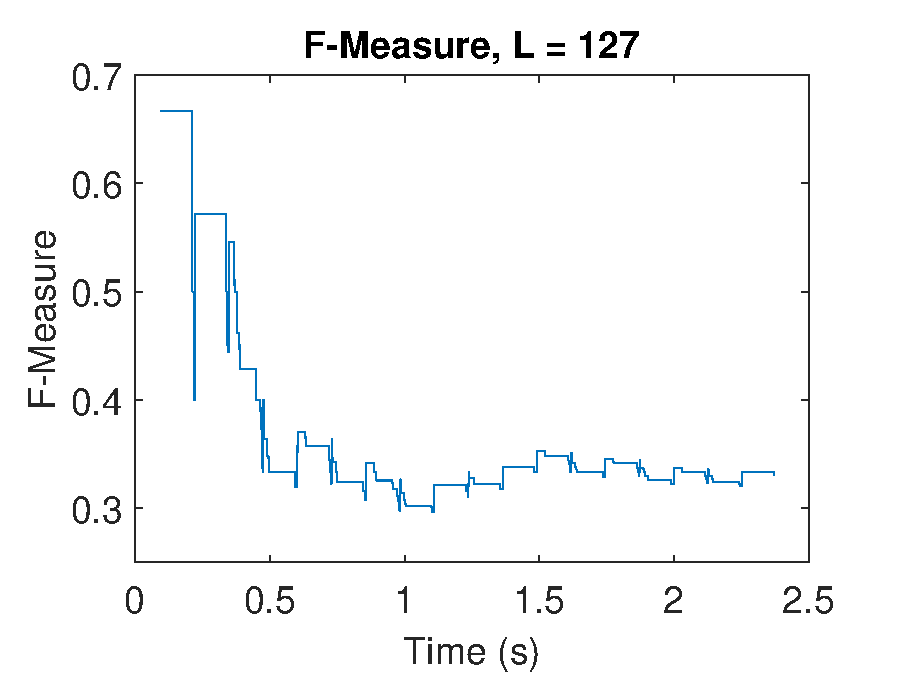
\includegraphics[width=\textwidth]{chapters/evaluation-chapters/hardware/dc/f-measure-dc-testbed-n=7.eps}
  	\caption{F-Measure of DC testbed correlation (\autoref{fig:correlation-dc-testbed-n=7}), with sequence length of 127.}
  	\label{fig:f-measure-dc-testbed-n=7}
  \end{minipage}
  \hfill
  \begin{minipage}[b]{0.49\textwidth}
    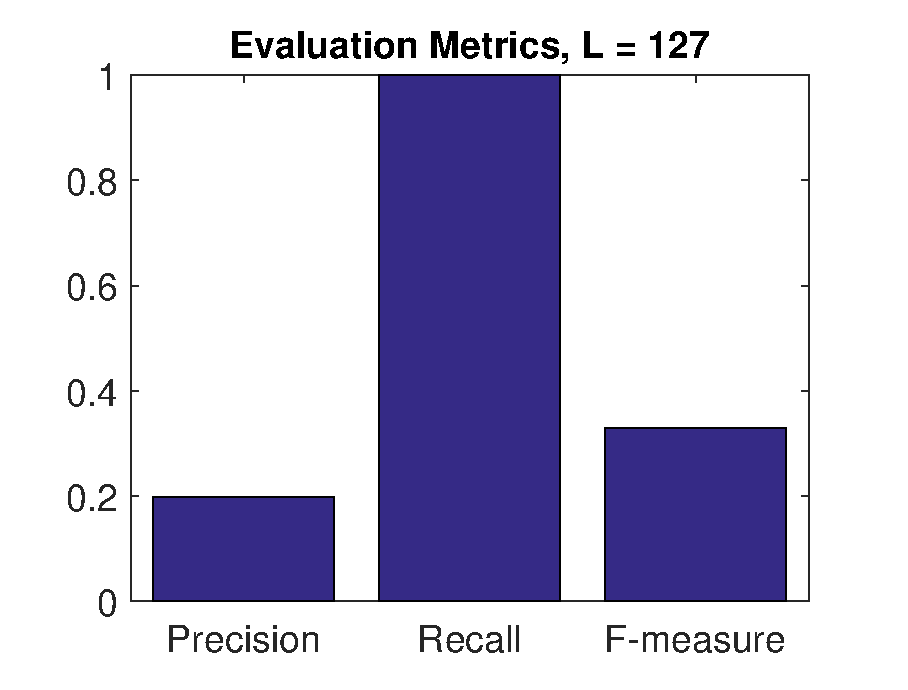
\includegraphics[width=\textwidth]{chapters/evaluation-chapters/hardware/dc/eval-metrics-dc-testbed-n=7.eps}
    \caption{Evaluation metrics of DC testbed correlation (\autoref{fig:correlation-dc-testbed-n=7}), with sequence length of 127.}
    \label{fig:eval-metrics-dc-testbed-n=7}
  \end{minipage}
\end{figure}